% SPDX-License-Identifier: MIT
% Copyright (c) 2026 LogNovations Holdings LLC
%
% Template of the paper. Every measured result is a placeholder into
% results.json, filled by scripts/make_paper.py. Edit this file, not paper.tex.
\documentclass[11pt]{article}
\usepackage[T1]{fontenc}
\usepackage[utf8]{inputenc}
\usepackage{lmodern,microtype}
\usepackage[a4paper,margin=2.4cm]{geometry}
\usepackage{graphicx,booktabs,amsmath,amssymb,xcolor,caption,enumitem,array}
\usepackage[superscript,biblabel]{cite}
\usepackage[hidelinks]{hyperref}
\pdfinfoomitdate=1 \pdftrailerid{} \pdfsuppressptexinfo=-1
\captionsetup{font=small,labelfont=bf}
\setlength{\parskip}{0.45em}
\setlength{\parindent}{0pt}
\raggedbottom
\renewcommand{\arraystretch}{1.15}
\newcommand{\arm}[1]{\textsc{#1}}

\title{\textbf{A pre-registered test of match-length features for certified selective acceptance of language-model outputs}}
\author{Chelsea McElveen\\[2pt]{\small LogNovations Holdings LLC}}
\date{12 November 2026}

\begin{document}
\maketitle

\begin{abstract}
\noindent Deployed language models need rules for deciding which outputs can be accepted without review. A threshold on a risk score, calibrated on labelled data, can carry a finite-sample bound on the error rate among accepted outputs. The share of outputs such a rule accepts, its certified coverage, then measures what a score is worth. We tested, under a pre-registration fixed before any calibration or test label was read, whether statistics of the lengths of matches between an output and its source context add certified coverage to a strong combination of existing scores. On the RAGTruth corpus they did not reach the bar set in advance. At an error level of 0.10 the baseline certified 8.84 points of coverage and the baseline with the features 8.02: a gain of $-0.82$ points (95\% interval, $-9.28$ to $+8.21$) against a bar of 10.78. Ranking metrics, which resolve smaller differences, did not move (change in AUROC, $-0.0021$; 95\% interval, $-0.0056$ to $+0.0014$). The features alone do rank errors (AUROC, 0.750; 0.459 with shuffled sources), about as well as word $n$-gram overlap and at a small fraction of the computing cost of a neural groundedness model. The endpoint was the binding constraint: its noise floor exceeded the baseline's own coverage. We release the pre-registration, the code, every record and an adversarial audit.
\end{abstract}

\section*{Introduction}

Large language models produce fluent text that is sometimes unsupported by, or in conflict with, the material they were given. In the corpus studied here, which holds responses of six models to question-answering, summarization and data-to-text prompts\cite{ragtruth}, a share of 0.46 of the test responses carries at least one annotated error. Many scores have been proposed to flag such responses, among them agreement between resampled outputs\cite{selfcheck}, dedicated groundedness classifiers\cite{minicheck} and entropy over meanings\cite{semanticentropy}. They are usually compared by how well they rank errors.

A ranking does not tell a deployer what to do. What is needed is a rule: accept an output when its score is below a threshold and defer it otherwise, with a known bound on how often an accepted output is wrong. Selective classification\cite{geifman} and distribution-free risk control\cite{ltt} supply such rules. In the form used here\cite{mcelveen}, a threshold is chosen on a labelled calibration sample so that, with probability at least $1-\delta$, the error rate among accepted outputs is at most $\alpha$, provided that calibration and deployment data are exchangeable. The share of outputs that the rule accepts is its \emph{certified coverage}. This is the operational value of a score: a better score lets more outputs through at the same guaranteed error rate. The bound is on an error rate, and it holds under exchangeability. It does not verify that any particular output is true.

We asked whether a family of cheap, model-free statistics adds certified coverage. For each position of an output, take the length of the longest substring starting there that also occurs in a reference text. This match-length profile underlies relative Lempel--Ziv parsing\cite{zivmerhav,barnfield} and match-length entropy estimation\cite{kontoyiannis}, and it is related to compression-based similarity\cite{ncd}. With the source context as the reference (\arm{source}), the profile measures how much of an output is reproduced from its source, and at what scales. With the output's own prefix as the reference (\arm{self}) it measures internal repetition, and with other samples drawn for the same prompt (\arm{resample}) it measures agreement between samples.

The hypotheses, their prior probabilities, the calibrator and the decision rule were fixed in writing before the study began. The data, the splits, the baselines and the analysis were then fixed in a pre-registration, which was approved and tagged before any calibration or test label was read. The primary hypothesis, H1, was that \arm{source} features add certified coverage over the best combination of baselines; its prior probability of being supported was put at 35--55\%. H3, that \arm{self} features do, was expected to fail (5--15\%). H2, for \arm{resample} features, was given 2--8\%.

H1 was not supported. Under the pre-registered rule its outcome is FAIL, which means that the gain is below the bar, not that the features carry no information. They do carry information, but the baselines already hold it. The study also showed, before any tested model was fitted, that certified coverage at this sample size is too coarse an endpoint to resolve gains of the size it was asked to judge. We report that finding with the same weight as the null result, because it bears on how scores of this kind should be evaluated.

\section*{Results}

\subsection*{Design}

RAGTruth\cite{ragtruth} holds responses of six language models to the same prompts, with human annotation of unsupported or conflicting spans. A response counts as an error when it has at least one annotated span. Sources were assigned by hash to six parts, so that the six responses to a source always share a part: two for fitting and selecting models, two for rehearsing the analysis on open data, and a calibration sample (CAL; 3,024 responses of 504 sources) and a test sample (TEST; 1,584 responses of 264 sources) whose labels were not read until the pre-registration was tagged (Extended Data Table~\ref{tab:splits}).

The baseline arm, \arm{baseline}, is a model over 25 columns: output length, the share of the output's word $n$-grams absent from the source, ROUGE-L against the source, the support scores of a groundedness classifier\cite{minicheck}, normalized compression distance\cite{ncd} with two compressors, and three covariates recorded with each response (generator, task type and temperature). The tested arms add the 16 \arm{source} features or the 16 \arm{self} features. Every arm was fitted with the same search over 24 model configurations and the same seed, and was frozen before the sealed labels were read.

Each arm's risk score was calibrated separately for each of the six generators, at confidence $\delta/6$ with $\delta = 0.05$, over a fixed grid of 20 thresholds. Certified coverage is the share of all test responses that the six thresholds accept, in percentage points. For short, we say that a generator is certified when a threshold was certified for its outputs; nothing is certified about a generator itself. The primary error level, $\alpha = 0.10$, was chosen by a rule written before any rehearsal: the strictest of 0.01, 0.05 and 0.10 at which \arm{baseline} certified at least 5 points on open data.

The decision rule was given in advance. BAR is the smaller of 5 points and 10\% of the coverage that \arm{baseline} leaves uncertified. FLOOR is the larger of 2 points and the 99th percentile of the gap between two refits of the same baseline (an A/A test). BAR is raised to FLOOR if it is below it. The outcome is PASS when the gain is at least BAR and its whole 95\% interval lies above FLOOR, FAIL when the upper end of the interval is below BAR, and INCONCLUSIVE otherwise.

\subsection*{The endpoint is coarse at this sample size}

In the open-data rehearsal \arm{baseline} certified 9.15 points of coverage, all of it from one generator. Because certification of a generator is all or nothing, two refits of the same model differ by a whole generator's share when one of them falls just short. In 1,000 A/A runs the absolute gap had a median of 1.28 points and a 99th percentile of 10.78 (Fig.~\ref{fig:endpoint}a). FLOOR, and with it BAR, was therefore 10.78 points: more than the baseline's whole coverage.

A power simulation at the CAL and TEST sizes followed (Fig.~\ref{fig:endpoint}b). When the true gain equalled BAR, none of 300 replications had its whole interval above FLOOR. PASS became likely (probability 0.89) only at a true gain of 21.6 points, more than twice the baseline's coverage, and for true gains between about 5 and 16 points the rule returned INCONCLUSIVE in most runs. The study's rules required it to stop at this point and ask. The study's owner was shown the result and chose to proceed with the design as written. No model with a tested feature had been fitted at that time, and how each outcome would be read was written into the pre-registration then: FAIL would be reported as ``the gain is below BAR'', which includes a real but smaller gain, and would not be described as evidence that the features carry no signal.

The simulation did not include a gain of zero. A probe added after the independent audit did: on 300 pairs of refits with no true gain, the rule returned FAIL for a share of 0.80 and INCONCLUSIVE for 0.20. FAIL is thus the likely outcome of this design both when there is no gain and when there is a gain of a few points, and the design cannot tell them apart.

\begin{figure}[t]
\centering
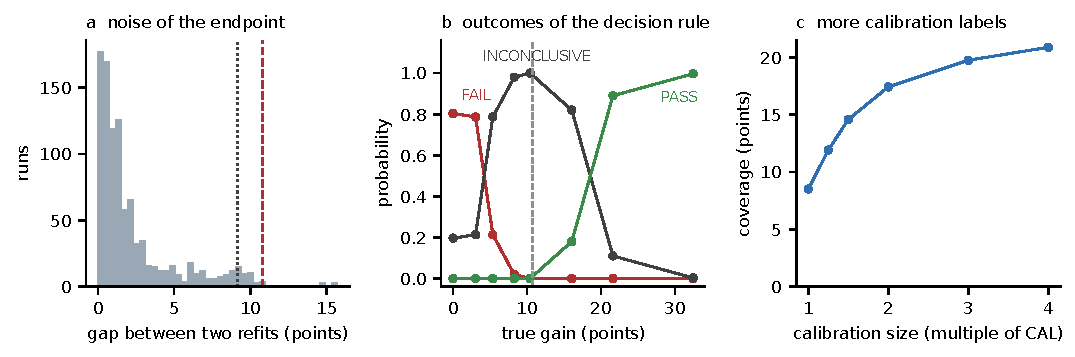
\includegraphics[width=\textwidth]{figures/fig1_endpoint.pdf}
\caption{\textbf{What the certified-coverage endpoint can resolve.} \textbf{a}, Absolute difference in certified coverage between two refits of the frozen \arm{baseline} configuration, 1,000 runs on open data. Dashed line, FLOOR, the 99th percentile; dotted line, the baseline's own coverage. \textbf{b}, Probability of each outcome of the decision rule against the true gain, by simulation at the calibration and test sizes (300 replications per point). The point at zero is the probe with no true gain. Dashed line, BAR. \textbf{c}, Mean certified coverage of \arm{baseline} on TEST when CAL is resampled, with replacement, to larger sizes (1,000 draws per point; a bootstrap estimate, not a measurement with new labels).}
\label{fig:endpoint}
\end{figure}

\subsection*{Primary result}

The confirmatory analysis read CAL and TEST once (Table~\ref{tab:main}, Fig.~\ref{fig:gains}). At $\alpha = 0.10$, \arm{baseline} certified 8.84 points of coverage and \arm{baseline+source} 8.02. The gain is $-0.82$ points, with a 95\% interval of $-9.28$ to $+8.21$. The upper end of the interval is below BAR (10.78 points), so the outcome for H1 is FAIL. As fixed in advance, this is read as: the gain is below 10.78 points. That includes a real but smaller gain.

Both arms certified one generator, GPT-4, and no other. \arm{baseline} did so at a rank threshold of 0.55 and \arm{baseline+source} at 0.50; the gain is that one step of the grid. No arm certified anything at $\alpha = 0.05$ or $0.01$. The error rate among accepted test outputs was 0.071 and 0.079, below $\alpha$.

H3 also failed. \arm{baseline+self} certified no generator, so its gain is the negative of the baseline's whole coverage ($-8.84$ points; interval, $-9.15$ to $+9.47$; Holm-adjusted $P = 1.00$). This point estimate is not a measured loss caused by the features: under one of two alternative definitions of the loss the same arm's gain was $+3.91$ points (Extended Data Table~\ref{tab:loss}). H2 could not be tested under the rule. Its dataset\cite{selfcheck} yields 52 independent calibration items, and with 52 error-free items the calibrator's bound is 0.1088, above every error level of the study. This follows from sample size and was established before any outcome was seen. Because the outcome for H1 was not INCONCLUSIVE, the single replication that the design reserved for that case was not run, and its data were never parsed.

\begin{table}[t]
\centering
\small
\caption{\textbf{Confirmatory result at $\alpha = 0.10$, $\delta = 0.05$.} Thresholds were certified on CAL and coverage was measured on the 1,584 responses of TEST. Gains are relative to \arm{baseline}, with 95\% intervals from a paired bootstrap of 10,000 draws of whole sources within task type. BAR $=$ FLOOR $= 10.78$ points.}
\label{tab:main}
\footnotesize
\setlength{\tabcolsep}{4.5pt}
\begin{tabular}{@{}lrrrlll@{}}
\toprule
Arm & \shortstack[r]{Coverage\\(points)} & \shortstack[r]{Accepted\\outputs} & \shortstack[r]{Error rate,\\accepted} & \shortstack[l]{Certified\\(threshold)} & \shortstack[l]{Gain, points\\(95\% interval)} & Outcome \\
\midrule
BASELINE & 8.84 & 140 & 0.071 & GPT-4 at 0.55 & reference & -- \\
BASELINE+SOURCE & 8.02 & 127 & 0.079 & GPT-4 at 0.50 & $-0.82$ ($-9.28$ to $+8.21$) & FAIL \\
BASELINE+SELF & 0.00 & 0 & -- & none & $-8.84$ ($-9.15$ to $+9.47$) & FAIL \\
\bottomrule
\end{tabular}
\end{table}

\begin{figure}[t]
\centering
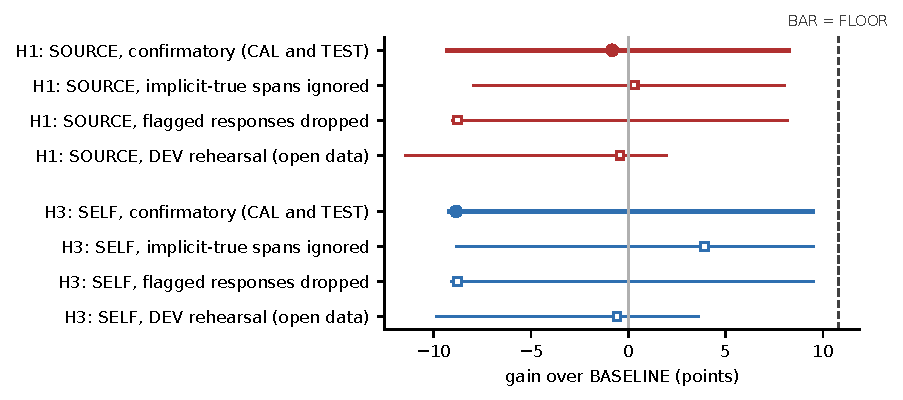
\includegraphics[width=0.78\textwidth]{figures/fig2_gains.pdf}
\caption{\textbf{Gains in certified coverage against the bar.} Point estimates and 95\% bootstrap intervals for H1 and H3. Filled circles, the confirmatory analysis. Open squares, three analyses that are not confirmatory: two alternative definitions of the loss (exploratory) and the rehearsal on open data. Dashed line, BAR $=$ FLOOR. Every upper end is below BAR. The point estimates move by up to a whole generator's share between analyses.}
\label{fig:gains}
\end{figure}

\subsection*{Ranking metrics did not move}

Ranking metrics were pre-registered as secondary, with the statement that they cannot change the outcome of H1 and are not support for it. They resolve differences that the endpoint cannot (Table~\ref{tab:ranking}, Fig.~\ref{fig:risk}). Adding the \arm{source} features changed AUROC on TEST by $-0.0021$ (95\% interval, $-0.0056$ to $+0.0014$), and adding the \arm{self} features changed it by $+0.0007$ ($-0.0021$ to $+0.0036$). These metrics pool the six generators, and \arm{baseline} is given the generator, whereas certification depends on ranking within a generator. Read off the recorded risk--coverage curves, the error rates among the lowest-risk quarter, half and three quarters of each generator's outputs differed between arms by a few errors in either direction, with no arm ahead (exploratory).

For H2's dataset, a ranking analysis stood in for the test that could not be run. On 197 test sentences of 25 passages, adding the 16 \arm{resample} features to a baseline that includes a resampling-based consistency score\cite{selfcheck} changed AUROC by $-0.0014$ ($-0.0295$ to $+0.0307$).

\begin{table}[t]
\centering
\small
\caption{\textbf{Ranking of errors on TEST.} An error is the positive class; AUPRC is average precision. Differences are from \arm{baseline}, with 95\% intervals from 10,000 paired bootstrap draws of whole sources within task type. Secondary metrics.}
\label{tab:ranking}
\begin{tabular}{@{}lrlrl@{}}
\toprule
Arm & AUROC & Difference (95\% interval) & AUPRC & Difference (95\% interval) \\
\midrule
BASELINE & 0.8851 & reference & 0.8726 & reference \\
BASELINE+SOURCE & 0.8830 & $-0.0021$ ($-0.0056$ to $+0.0014$) & 0.8733 & $+0.0007$ ($-0.0065$ to $+0.0075$) \\
BASELINE+SELF & 0.8859 & $+0.0007$ ($-0.0021$ to $+0.0036$) & 0.8711 & $-0.0015$ ($-0.0088$ to $+0.0048$) \\
\bottomrule
\end{tabular}
\end{table}

\begin{figure}[t]
\centering
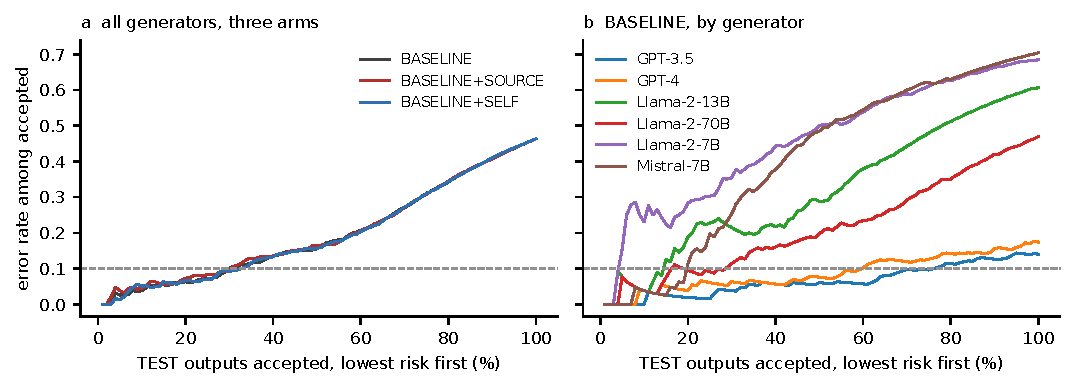
\includegraphics[width=\textwidth]{figures/fig3_risk_coverage.pdf}
\caption{\textbf{Risk--coverage curves on TEST.} Error rate among the accepted outputs when outputs are accepted in order of increasing risk score. \textbf{a}, The three arms over all generators; the curves nearly coincide. \textbf{b}, \arm{baseline} within each generator. Dashed line, $\alpha = 0.10$. These are empirical curves, not certified ones.}
\label{fig:risk}
\end{figure}

\subsection*{The features carry signal that the baselines already hold}

By themselves the \arm{source} features do rank errors. A logistic model on the 16 columns had an AUROC of 0.750 on TEST, against 0.634 for output length alone and 0.503 for a random score. The ranking depends on the source. When each output was paired with the source of another item of the same task type, the same model's AUROC fell to 0.459. It is not a length effect either: within quintiles of output length the model's AUROC lay between 0.706 and 0.751. The \arm{self} features were weaker (0.666).

Existing scores do as well (Table~\ref{tab:single}). The strongest single \arm{source} features are coverage of the output by matches of at least 8 bytes and the number of relative Lempel--Ziv phrases per byte. The share of novel word 1-grams, a baseline that is simpler to compute, matches them, and the groundedness classifier is somewhat stronger. Only the short scales matter: coverage by matches of 128 bytes or more is uninformative on outputs of this length (on the selection split, the middle three fifths of outputs are between 510 and 1,075 bytes long).

The scores differ far more in cost than in ranking power (Fig.~\ref{fig:cost}). The \arm{source} profile took 0.53 seconds per megabyte of input on one CPU thread in a Python reference implementation, and the lexical baselines 0.24. The groundedness classifier took 423 seconds per megabyte on the same machine's GPU. On TEST the model on the \arm{source} features alone certified the same coverage as \arm{baseline+source}, 8.02 points; on the open-data rehearsal it certified 0.00 against 9.15 for \arm{baseline} (Extended Data Table~\ref{tab:alone}). That comparison was not pre-registered, both differences lie inside the noise floor, and we draw no conclusion from it.

\begin{table}[t]
\centering
\small
\caption{\textbf{Strongest single scores on TEST.} The three \arm{source} features and the three baseline columns farthest from 0.5. The fourth column takes each score in whichever direction ranks errors higher, a choice made after seeing TEST that flatters every row equally. Exploratory.}
\label{tab:single}
\begin{tabular}{@{}llrrl@{}}
\toprule
Column & Family & AUROC & \shortstack[r]{AUROC, direction\\chosen afterwards} & Higher for \\
\midrule
\texttt{source.cov\_k8} & SOURCE feature & 0.251 & 0.749 & correct outputs \\
\texttt{source.rlz\_phrases\_per\_symbol} & SOURCE feature & 0.748 & 0.748 & errors \\
\texttt{source.cov\_k4} & SOURCE feature & 0.266 & 0.734 & correct outputs \\
\texttt{gnd.mean} & baseline & 0.219 & 0.781 & correct outputs \\
\texttt{gnd.frac\_unsupported} & baseline & 0.772 & 0.772 & errors \\
\texttt{base.novel\_1gram} & baseline & 0.760 & 0.760 & errors \\
\bottomrule
\end{tabular}
\end{table}

\begin{figure}[t]
\centering
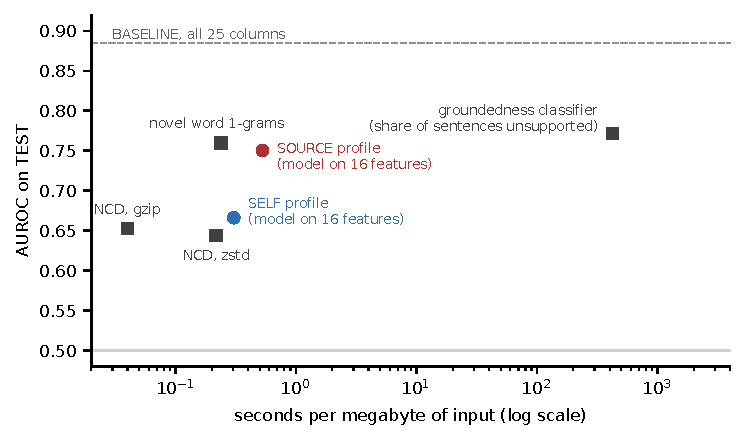
\includegraphics[width=0.66\textwidth]{figures/fig4_signal_cost.pdf}
\caption{\textbf{Ranking power against computing cost.} AUROC on TEST against seconds per megabyte of input. Circles, logistic models on the 16 features of a match-length profile; squares, single baseline scores. Dashed line, the full \arm{baseline}, whose cost is dominated by the groundedness classifier. CPU scores were timed on one thread; the groundedness classifier was timed on a GPU for 583 of the sealed items. Exploratory.}
\label{fig:cost}
\end{figure}

\subsection*{Controls, guarantee checks and stress analyses}

With calibration and test labels permuted within generator, no score certified any coverage in 1,000 permutations, and a random score certified none with the true labels. These two controls could hardly have come out otherwise, because every generator's error rate exceeds $\alpha$; they would catch a calibrator that certifies without evidence and little else. The shuffled-source control above is the informative one.

The calibrator's guarantee was checked in two ways. On synthetic data with risk known in closed form, the true risk among accepted outputs never exceeded $\alpha$ in 10,000 draws. On real data, CAL and TEST were pooled and re-split 1,000 times, and no re-split was flagged by the pre-registered test. Both checks can detect only a gross failure. Where exchangeability was broken on purpose, the bound did not hold: with thresholds certified on two task types and applied to the third, \arm{baseline} accepted 13 data-to-text outputs with an error rate of 0.46.

The outcome did not depend on the definition of the loss, but the point estimates did. Under two exploratory variants the rule again returned FAIL for H1 and H3, while H1's gain ranged from $-8.77$ to $+0.32$ points (Fig.~\ref{fig:gains}). Computing the features over word tokens in place of bytes left AUROC unchanged. When 300 test outputs were reworded by a small open-weight model and rescored, \arm{baseline} still accepted 16 of the 21 outputs it had accepted, and \arm{baseline+source} 10 of 21. Features that measure verbatim overlap are, as expected, sensitive to rewording; the sample is small and has no labels, so whether the reworded outputs were as correct as the originals is not known.

\subsection*{Calibration labels were worth more than features}

At the actual size of CAL, resampling it certified any coverage at all in a share of 0.76 of draws, with a mean of 8.52 points. Resampled to twice the size, \arm{baseline} alone certified 17.42 points on average, and at four times the size 20.87 (Fig.~\ref{fig:endpoint}c). No feature in this study moved coverage by a comparable amount.

\subsection*{Independent audit}

A reviewer that had not seen the implementation was instructed to refute the result without reading a sealed label (Methods). It recomputed the bar, the noise floor and both outcomes from the committed records, refitted the frozen models from open data to the same file hashes, and found no path by which a calibration or test label could have reached a feature, a model or a threshold other than through calibration. It concluded that the outcomes stand. It also made thirteen findings, which led to corrections and to three additional analyses. Two bear on interpretation. First, the temperature recorded with each response is strongly related to the label within four of the six generators (within-generator AUROC of temperature alone, between 0.26 and 0.34, where a value below 0.5 means that a higher temperature goes with fewer errors). If that relation is an artefact of how the corpus was produced, \arm{baseline} is stronger here than a deployable baseline would be. Refitted on open data without the column, \arm{baseline} ranked worse, and adding the \arm{source} features still did not improve it (change in AUROC, $-0.0019$; $-0.0057$ to $+0.0020$; Extended Data Table~\ref{tab:temperature}). Second, that the confirmatory analysis ran exactly once cannot be proved from the repository alone; it rests on the run ledger and on the command log of the session.

\section*{Discussion}

The question was whether match-length statistics add certified coverage to a strong baseline. Under a rule fixed in advance, the answer on this corpus is that any gain is below 10.78 points, and the more sensitive ranking metrics give no sign of a gain of any size. The \arm{self} features added nothing, and the \arm{resample} features could not be tested for certification.

The features are not noise. Against the source they rank errors on their own, the ranking disappears when sources are shuffled, and it survives conditioning on length. But the share of novel word $n$-grams does the same job. The simplest account, which we did not test, is that match-length statistics against a source measure verbatim overlap, and that lexical baselines already measure verbatim overlap. On short outputs the multi-scale structure of the profile has little room to add anything: only matches of a few bytes to a few tens of bytes were informative.

Three observations may be of use beyond this feature family. First, certified coverage is a demanding endpoint. With about 500 calibration items per stratum and error rates of 14\% and more, only one stratum was certified, the noise between two refits of one model exceeded the coverage being compared, and a rule built on that noise returned INCONCLUSIVE one time in five when there was nothing to find. Studies that compare scores by certified coverage should report an A/A noise floor and the rule's behaviour under no gain, as well as power. Second, on these data the size of the calibration sample mattered more than the choice of score. Third, lexical overlap with the source, however it is computed, ranked errors nearly as well as a neural groundedness classifier, in roughly one thousandth of the computing time and on one CPU thread in place of a GPU. Whether a cheap score can stand in for, or be cascaded before, an expensive one at a guaranteed error rate is a different hypothesis from the one tested here, and would need its own pre-registered test with adequate power.

The study has limits. It has one confirmatory corpus, six generators, three task types and English text. Four baselines named in advance (verbalized confidence, token log-probability, token entropy and semantic entropy\cite{semanticentropy}) need access to the generator and could not be run, so \arm{baseline} is the best combination of what could be run. It includes a covariate, temperature, whose relation to the label in this corpus is unexplained. One pair of similar sources sits across CAL and TEST, below the pre-registered similarity threshold. The percentile bootstrap of a step-function statistic need not have nominal coverage. The guarantee is marginal over accepted outputs and conditional on exchangeability, and it was checked empirically, not re-derived. The replication reserved for an INCONCLUSIVE outcome was specified but never implemented, because it was not triggered. The pre-registration was tagged in a private repository and was not deposited with a third party before the confirmatory run, so its priority rests on that repository's history. The analysis and this manuscript were produced with an AI system and audited by a second instance of the same system; no human statistician has reviewed them (Methods).

A null result under a pre-registration is informative in proportion to what was fixed in advance and what can be checked afterwards. Everything needed to check this one is public: the plan as tagged, each record with the commit that produced it, the ledger of reads of the sealed data, the incidents, and the reviewer's findings with what was done about each.

\section*{Methods}

\subsection*{Pre-registration and conduct}
The study's owner fixed the hypotheses, their prior probabilities, the calibrator and the decision rule in a written brief, together with rules of conduct: no number, dataset or citation may be fabricated or estimated; the decision rule, endpoint, datasets and splits may not change after calibration or test data are seen; no baseline may be weakened; and the result is to be described as a score for selective acceptance with an error bound that holds under exchangeability. The pre-registration (\texttt{PREREGISTRATION.md} in the repository) was written from that brief, approved by the owner and tagged before any CAL or TEST label was read. It is byte-identical to the tagged version. Nothing that was analysed deviates from it. One deviation concerns what is reported: the plan said that a second, proprietary implementation of the profile would be reported for agreement and throughput, and the author decided before publication not to publish its measurements; no result here depends on it. Three incidents were recorded: a label-free scoring run was killed by memory exhaustion and resumed, with a check that rescored items matched; and two files were rewritten and restored by checks run just before and just after the confirmatory analysis. None read a sealed label.

\subsection*{Data}
RAGTruth\cite{ragtruth} was read from its public repository at a pinned commit. One response is one item. The loss is 1 when a response has at least one annotated span of any type, and no response was excluded. The reference for the \arm{source} profile is the prompt, the exact text given to the generator. Sources whose content had a Jaccard similarity of at least 0.9 on lower-cased word 5-grams were treated as one, which removed one source. The corpus authors' own test split (2,700 responses) was reserved for a single replication and never parsed. The remaining 2,514 sources (15,084 responses) were assigned to six splits by a hash of the source identifier, with fractions 0.30, 0.10, 0.20, 0.10, 0.20 and 0.10. For H2, the WikiBio GPT-3 hallucination dataset\cite{selfcheck} was split by passage in the same way; its loss is 1 unless a sentence is labelled accurate. The labels of the calibration and test splits were dropped as the tables were built and written to no file. The study's code reads them only through a guard that requires an explicit flag, the pre-registration tag and a clean working tree, and that appends each read to a ledger. The guard is a procedural control, not a technical barrier.

\subsection*{Features under test}
For a byte string $T$ of length $n$ and a reference $R$, the profile is $L[i]$, the length of the longest substring of $T$ starting at $i$ that occurs in $R$. Sixteen features were computed from each profile: the share of positions covered by a match of length at least $k$, for $k = 1, 2, 4, \dots, 1024$; the number of phrases in the greedy relative Lempel--Ziv parse\cite{zivmerhav}, and that number per byte; the longest common substring, and its share of $n$; and a match-length entropy estimate\cite{kontoyiannis}. The entropy estimate with a fixed reference replaces the window of previous symbols in the source theorem by the reference; that substitution is ours, and the quantity is used as a score, not as an estimate. Profiles were computed with a suffix automaton\cite{blumer} and tested against brute-force definitions. Normalized compression distance\cite{ncd} is a baseline, not a tested feature. Code that computes a score has no parameter through which a label could arrive, and tests enforce this.

\subsection*{Baselines and models}
The baseline columns are listed in Results. The groundedness classifier is MiniCheck-DeBERTa-v3-Large\cite{minicheck} at a pinned revision, applied by this study's code as its reference inference code applies it: each sentence of a response is a claim, scored against chunks of the source, and the columns are the minimum support, the mean support and the share of sentences with support below 0.5. Each arm's model was chosen from 8 L2-regularized logistic regressions and 16 gradient-boosted tree models by log loss on a selection split, after fitting on the training split, with one seed for all arms. For the H2 dataset, the consistency baseline is SelfCheckGPT with an NLI model\cite{selfcheck}; its published area under the precision--recall curve of 92.50 was reproduced on the open splits as 92.78, within a tolerance fixed beforehand.

\subsection*{Calibration and certified coverage}
The calibrator is \texttt{calibrate\_bonferroni} from the companion work\cite{mcelveen}, used at a pinned commit and not reimplemented. For each of $K$ grid thresholds it computes a one-sided Clopper--Pearson\cite{clopper} upper bound, at level $1-\delta/K$, on the error rate among accepted calibration items, and returns the largest threshold whose bound is at most $\alpha$, or none. Each risk score was first mapped to $[0,1]$ by its empirical distribution on the selection split, separately for each generator, and the grid was 20 uniform thresholds. Because the six responses to a source are not independent, calibration was run once per generator at $\delta/6$, so that all six certificates hold together with probability at least $1-\delta$. With this design the smallest error-free accepted set that can be certified has 74 items at $\alpha = 0.10$, 152 at 0.05 and 775 at 0.01; with 504 calibration sources per generator, nothing can be certified at 0.01.

\subsection*{Endpoint, interval and decision rule}
The endpoint is the certified coverage of the tested arm minus that of \arm{baseline}, in points, at the primary $\alpha$, with thresholds certified on CAL and coverage measured on TEST. The 95\% interval is the 2.5th to 97.5th percentile of 10,000 paired bootstrap draws; each draw resamples whole sources with replacement within task type, in CAL and in TEST, and recertifies both arms on the same resample. The rule is given in Results; the absolute A/A gap was used, and inequalities are strict. For the secondary family (H2, H3), the $P$ value of a gain is the share of bootstrap draws at or below FLOOR, with Holm's adjustment\cite{holm}; H2 entered with $P = 1$.

\subsection*{Controls and additional analyses}
All were pre-registered unless marked exploratory in Results, and all were run after the confirmatory record had been committed. They comprise the permuted-label, random-score and shuffled-source controls; coverage of output length alone and ranking within length quintiles; the two guarantee checks; two alternative definitions of the loss; resampling of the calibration sample to larger sizes; breakdowns by generator and task type; calibration across task types; features over word tokens; and rewording of 300 test outputs by an open-weight model run locally. Three probes were added after the audit and use open or label-free data only: similar sources across splits, the temperature covariate, and the decision rule applied to pairs of refits with no true gain.

\subsection*{Reads of the sealed data}
In the study, the calibration and test labels of RAGTruth were read twice each, by the confirmatory analysis and by the controls, and the test labels of the H2 dataset once. A reproduction in a clone later read them again. The ledger records each read with its commit and purpose.

\subsection*{Reproducibility}
One command rebuilds every record from the raw files, which are pinned by commit and checksum. Every result in this paper is read from a single file of records (\texttt{results.json}) when the paper is rendered, and each record carries the commit that produced it. One reproduction was run, in a fresh clone on the machine the study ran on. Of 17 records, 17 were identical to the study's apart from provenance stamps, ledger rows and timings. In its own clone the reproduction read the calibration labels 2 times and test labels 3 times, after every result reported here had been committed. The scores of the two neural baselines were reused in that reproduction, not recomputed. The test suite passes in a container built from a locked environment.

\subsection*{Independent audit}
A second instance of the AI system that built the study was started without the builder's history. It was given the brief, the repository and the instruction to refute the result, with attention to leakage, reuse of the test data, thresholds chosen from the sample, weak baselines, duplicate groups, drift of the label definition, selective use of data, overstated claims and the statistics. It was not allowed to read a sealed label. Its report, its thirteen findings and the response to each are in Section~8 of \texttt{REPORT.md} in the repository. The corrections it prompted were made by the builder and were not audited again.

\subsection*{Use of an AI system}
The author posed the question, fixed the hypotheses, priors, calibrator and decision rule, decided the open questions at the gates the brief defined (among them the reserved replication set, the dataset for H2, the computing budget and whether to proceed after the power analysis), approved the pre-registration, and is responsible for the work. The code, the pre-registration document, the analyses, the audit and the text of this manuscript were produced by an AI system (Claude; Anthropic) working under those instructions. No human statistician has reviewed the work.

\subsection*{Citations}
The definitions used were read in the primary sources for refs.~\citenum{mcelveen}, \citenum{zivmerhav} and \citenum{kontoyiannis}, and in the arXiv version for ref.~\citenum{ncd}; ref.~\citenum{barnfield} was read as a restatement of the parse of ref.~\citenum{zivmerhav}. Facts quoted from refs.~\citenum{ragtruth} and \citenum{selfcheck} were read in those papers. Refs.~\citenum{minicheck}, \citenum{semanticentropy}, \citenum{geifman}, \citenum{ltt}, \citenum{blumer}, \citenum{clopper} and \citenum{holm} are cited from their bibliographic records. Those articles were not read for this study, and nothing that rests on them was used without a separate check: the calibrator's bound was read in its source code, and the suffix automaton and the Holm adjustment are tested against direct definitions.

\section*{Data availability}
RAGTruth and the WikiBio GPT-3 hallucination dataset are public. The repository pins the commit and the SHA-256 of every raw file and contains every derived record of the study.

\section*{Code availability}
The harness, the pre-registration, the records, the run ledger and the full report are at \url{https://github.com/chelsinchaos/match-length-selective-acceptance}, under the MIT licence. That repository is an export of the harness from the private repository in which the study was run; commit hashes in the records refer to the private repository, and a file in the export lists them.

\section*{Competing interests}
The author is the founder of LogNovations Holdings LLC, which develops a proprietary data codec. The features tested here are computed by an open reference implementation that does not use it. The study was run as an experiment in the open: the plan, the code, every record and the audit are public, whichever way the result came out.

\begin{thebibliography}{99}\small
\bibitem{ragtruth} Niu, C. et al. RAGTruth: a hallucination corpus for developing trustworthy retrieval-augmented language models. Preprint at arXiv:2401.00396 (2024).
\bibitem{selfcheck} Manakul, P., Liusie, A. \& Gales, M. J. F. SelfCheckGPT: zero-resource black-box hallucination detection for generative large language models. Preprint at arXiv:2303.08896 (2023).
\bibitem{minicheck} Tang, L., Laban, P. \& Durrett, G. MiniCheck: efficient fact-checking of LLMs on grounding documents. In \emph{Proc. EMNLP 2024} 8818--8847 (2024).
\bibitem{semanticentropy} Farquhar, S., Kossen, J., Kuhn, L. \& Gal, Y. Detecting hallucinations in large language models using semantic entropy. \emph{Nature} \textbf{630}, 625--630 (2024).
\bibitem{geifman} Geifman, Y. \& El-Yaniv, R. Selective classification for deep neural networks. Preprint at arXiv:1705.08500 (2017).
\bibitem{ltt} Angelopoulos, A. N., Bates, S., Cand\`es, E. J., Jordan, M. I. \& Lei, L. Learn then Test: calibrating predictive algorithms to achieve risk control. Preprint at arXiv:2110.01052 (2021).
\bibitem{mcelveen} McElveen, C. Explanation is not certification: information-theoretic limits of interpretability-based assurance for machine learning systems. Manuscript and code in the companion repository (2026).
\bibitem{zivmerhav} Ziv, J. \& Merhav, N. A measure of relative entropy between individual sequences with application to universal classification. \emph{IEEE Trans. Inf. Theory} \textbf{39}, 1270--1279 (1993).
\bibitem{barnfield} Barnfield, N., Grondin, R., Pozzoli, G. \& Raqu\'epas, R. On the Ziv--Merhav theorem beyond Markovianity. Preprint at arXiv:2310.01367 (2023).
\bibitem{kontoyiannis} Kontoyiannis, I., Algoet, P. H., Suhov, Yu. M. \& Wyner, A. J. Nonparametric entropy estimation for stationary processes and random fields, with applications to English text. \emph{IEEE Trans. Inf. Theory} \textbf{44}, 1319--1327 (1998).
\bibitem{ncd} Cilibrasi, R. \& Vit\'anyi, P. M. B. Clustering by compression. \emph{IEEE Trans. Inf. Theory} \textbf{51}, 1523--1545 (2005).
\bibitem{blumer} Blumer, A. et al. The smallest automaton recognizing the subwords of a text. \emph{Theor. Comput. Sci.} \textbf{40}, 31--55 (1985).
\bibitem{clopper} Clopper, C. J. \& Pearson, E. S. The use of confidence or fiducial limits illustrated in the case of the binomial. \emph{Biometrika} \textbf{26}, 404--413 (1934).
\bibitem{holm} Holm, S. A simple sequentially rejective multiple test procedure. \emph{Scand. J. Stat.} \textbf{6}, 65--70 (1979).
\end{thebibliography}

\clearpage
\section*{Extended Data}
\setcounter{table}{0}
\renewcommand{\tablename}{Extended Data Table}

\begin{table}[h]
\centering
\small
\caption{\textbf{Splits.} Groups are sources (RAGTruth) or passages (WikiBio GPT-3). The first four splits are open; the labels of CAL and TEST were sealed until the pre-registration was tagged. The calibration labels of WikiBio were never read.}
\label{tab:splits}
\begin{tabular}{@{}llrr@{}}
\toprule
Dataset & Split & Groups & Items \\
\midrule
RAGTruth & TRAIN & 747 & 4,482 \\
RAGTruth & DEV\_SELECT & 238 & 1,428 \\
RAGTruth & DEV\_CAL & 526 & 3,156 \\
RAGTruth & DEV\_TEST & 235 & 1,410 \\
RAGTruth & CAL & 504 & 3,024 \\
RAGTruth & TEST & 264 & 1,584 \\
WikiBio GPT-3 & TRAIN & 78 & 594 \\
WikiBio GPT-3 & DEV\_SELECT & 17 & 143 \\
WikiBio GPT-3 & DEV\_CAL & 41 & 326 \\
WikiBio GPT-3 & DEV\_TEST & 25 & 223 \\
WikiBio GPT-3 & CAL & 52 & 425 \\
WikiBio GPT-3 & TEST & 25 & 197 \\
\bottomrule
\end{tabular}
\end{table}

\begin{table}[h]
\centering
\small
\caption{\textbf{By generator, at $\alpha = 0.10$.} Accepted test outputs, with the error rate among them in parentheses. Exploratory.}
\label{tab:generators}
\begin{tabular}{@{}lrrlll@{}}
\toprule
Generator & \shortstack[r]{Test\\items} & \shortstack[r]{Error\\rate} & \arm{baseline} & \arm{baseline+source} & \arm{baseline+self} \\
\midrule
GPT-3.5 & 264 & 0.140 & 0 (--) & 0 (--) & 0 (--) \\
GPT-4 & 264 & 0.174 & 140 (0.071) & 127 (0.079) & 0 (--) \\
Llama-2-13B & 264 & 0.606 & 0 (--) & 0 (--) & 0 (--) \\
Llama-2-70B & 264 & 0.470 & 0 (--) & 0 (--) & 0 (--) \\
Llama-2-7B & 264 & 0.686 & 0 (--) & 0 (--) & 0 (--) \\
Mistral-7B & 264 & 0.705 & 0 (--) & 0 (--) & 0 (--) \\
\bottomrule
\end{tabular}
\end{table}

\begin{table}[h]
\centering
\small
\caption{\textbf{Sensitivity to the definition of the loss.} Certified coverage of the three arms in points, and gains with 95\% intervals. Both variants were named before the loss was fixed, and both are exploratory. The outcome under the rule is FAIL in every cell of the last two columns.}
\label{tab:loss}
\footnotesize
\setlength{\tabcolsep}{4.5pt}
\begin{tabular}{@{}lrrrll@{}}
\toprule
Loss & \arm{baseline} & \arm{+source} & \arm{+self} & H1 gain & H3 gain \\
\midrule
As pre-registered & 8.84 & 8.02 & 0.00 & $-0.82$ ($-9.28$ to $+8.21$) & $-8.84$ ($-9.15$ to $+9.47$) \\
Implicit-true spans ignored & 16.79 & 17.11 & 20.71 & $+0.32$ ($-7.95$ to $+8.02$) & $+3.91$ ($-8.84$ to $+9.53$) \\
Flagged responses dropped & 8.77 & 0.00 & 0.00 & $-8.77$ ($-9.02$ to $+8.19$) & $-8.77$ ($-9.07$ to $+9.52$) \\
\bottomrule
\end{tabular}
\end{table}

\begin{table}[h]
\centering
\small
\caption{\textbf{Models on one family of columns, on TEST at $\alpha = 0.10$.} The rows for output length and the random score were pre-registered; the rows for the tested features alone are additions. The model on the \arm{source} features certified GPT-4, as \arm{baseline} did. Exploratory.}
\label{tab:alone}
\begin{tabular}{@{}lrrrr@{}}
\toprule
Score & AUROC & \shortstack[r]{Coverage\\(points)} & Accepted & \shortstack[r]{Error rate\\among accepted} \\
\midrule
BASELINE (25 columns) & 0.885 & 8.84 & 140 & 0.071 \\
16 SOURCE columns (logistic) & 0.750 & 8.02 & 127 & 0.079 \\
16 SELF columns (logistic) & 0.666 & 0.00 & 0 & -- \\
Output length (3 columns) & 0.634 & 0.00 & 0 & -- \\
Random score & 0.503 & 0.00 & 0 & -- \\
\bottomrule
\end{tabular}
\end{table}

\begin{table}[h]
\centering
\small
\caption{\textbf{The temperature covariate, on open data.} Arms refitted on the training split with and without the temperature column, with the same search and seed, and evaluated on the open development test split. The refits with temperature select the frozen configurations. Exploratory; added after the audit.}
\label{tab:temperature}
\begin{tabular}{@{}lrrr@{}}
\toprule
Model & Columns & AUROC & \shortstack[r]{Coverage in the\\rehearsal (points)} \\
\midrule
BASELINE & 25 & 0.9062 & 9.15 \\
BASELINE without temperature & 24 & 0.8898 & 9.29 \\
BASELINE+SOURCE & 41 & 0.9051 & 8.72 \\
BASELINE+SOURCE without temperature & 40 & 0.8879 & 10.14 \\
\bottomrule
\end{tabular}
\end{table}

\end{document}
